\chapter[SCP-144 西藏通天绳]{
    SCP-144 Tibetan Rope to Heaven\\
    SCP-144 西藏通天绳
}

\label{chap:SCP-144}

\begin{figure}[H]
    \centering
    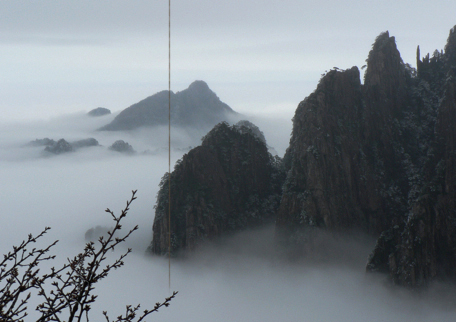
\includegraphics[width=0.5\linewidth]{images/SCP.144.jpg}
    \caption*{一张从最近的山峰上拍摄的SCP-144照片,在它下面的庙因为雾气而无法看见。}
\end{figure}

\bb{项目编号:}SCP-144

\bb{项目等级:}Safe

\bb{特殊收容措施:}SCP-144现阶段只需要一名SCP观察员进行观察并且对其状况进行实时更新。那些维持着该地点的西藏僧侣们都以一种与世隔绝的方式隐居着。大量的雾气浓缩在有着144存在的小山的周围,而它本身则坐落于两座高峰之间,分别是{[}数据删除]峰和{[}数据删除]峰。这些雾气几乎终年出现,并且144只有在3km的范围之内才能被肉眼所观察到。在中国政|府的帮助之下,半径70km以内的飞行行为都被严格限制了。

\bb{描述:}位于一座地处西藏小山山顶的僧院之中,SCP-144是一根紧绷的大麻绳,它只有1.2cm的直径,系在一个位于中庭地面的玉环上(这在研究员之中被称为“基点”)。而144的另一头则直直地向天延伸了数公里,现在被地球静止轨道卫星探测到结束于海拔39km的高空之中(延伸了22英里,在研究员之中这被称为“顶点”)。

一年之中有数次,一名僧侣将会在一个寻求灵魂启示的仪式之中顺着这根绳子上升数百米。僧侣们报告说时至今日,只有一名名为{[}数据删除]的僧侣在这个上升过程之中摔死了。数个世纪以来,数名攀爬者消失了,但是这些僧侣们都相信终有一天他们将会回来,为他们带来更多的智慧和启示。

碳-14测年法将这根绳子的时间回溯到了1400年前,基金会的人类学家相信这根绳子和攀爬它的仪式都是从已经去世的松赞干布王将佛教带入西藏的时候开始出现的。在那时,这根绳子只被认为有数公里长。随侍的僧侣说这个玉环是是在9世纪早期由赤祖德赞加上的,是为了防止季风将这根绳子带走并且在全国范围内吹动。一年之中有数次,住持将会将这根绳子从玉环上解下,然后再重新将其系上。研究已经证明,在最近几年,这根绳子都会向天伸展180cm,并且这个速率还在以1\slash 100 厘米\slash 年2的加速度加速着。因为只有数百米的绳子还在地上,这些僧侣们都不知道当这根绳子伸展到了终点时他们应该做什么。有的僧侣希望能够在这根绳子上接上新的部分,但是有的僧侣认为新的绳子不会有向旧的绳子那样的性质了。

研究者们无法解释这些植物纤维是怎样能够在外太空这样严苛的温度和环境下遗存1400年,还是保持这样紧绷不变的,并且还可以让人类攀爬,更不必说它本身所具有的巨大重量了(所有39km的绳子加起来的重量)。如果其顶点还在从地球上加速向太空伸张,那么是什么在拉着它也是未知的。

这根绳子的顶点只能从在地面部署的望远镜上拍摄到,照片显示144一直向上延伸,最终在一块类小行星的岩石周围停止了,这块岩石有数百米宽。卫星不能拍到顶点的另一面(“暗面”)。这是因为静止轨道卫星本来就是设计拍摄固定于地面的物体,或者是远距离太空物体而不是邻近的太空物体的。研究员在为什么对于其“暗面”拍摄的照片都是模糊一片并且不能聚焦不能达成一致意见,这使得其暗面现在还是未知的。

\bb{附录144-4:}数名D级人员被开出了如果他们能够爬到顶点,如果可能的话,再回来,他们将会得到立刻释放的承诺。虽然随侍于这根绳子的僧侣们提出了数个警告,但是他们没有施加任何阻力。

在接受了这一条件的6名人员之中,有4名最终回到了基点,抱怨着难以呼吸和空气缺乏。1名人员以致命的速度摔回了基点,推测是因为疲劳而最终松开了绳子,而最后一名到现在都没有回来。
